\PassOptionsToPackage{inline}{enumitem}
\documentclass[columns=3, numbered theorems=false]{mycheatsheet}

\usepackage{svg}
\usepackage{siunitx}
\usepackage[normalem]{ulem}
\usepackage{circuitikz}
\usepackage{xcolor}
\usepackage{mathtools}
\usepackage{esvect}

\usetikzlibrary{positioning}

\setlist{itemjoin={\hspace{1em}}}

\setlength{\parskip}{.5ex plus .5ex minus .2ex}

\renewcommand{\boldsymbol}[1]{\symbfit{#1}}

\AtBeginDocument{\let\div\divergence}

\newcommand{\ur}{\ensuremath{\vu{u}_\mathrm{r}}}
\newcommand{\uR}{\ensuremath{\vu{u}_R}}
\newcommand{\up}{\ensuremath{\vu{u}_\rho}}
\newcommand{\uphi}{\ensuremath{\vu{u}_\phi}}
\newcommand{\ux}{\ensuremath{\vu{u}_\mathrm{x}}}
\newcommand{\uy}{\ensuremath{\vu{u}_\mathrm{y}}}
\newcommand{\uz}{\ensuremath{\vu{u}_\mathrm{z}}}
\renewcommand{\r}{\ensuremath{\vu{r}}}

\renewcommand{\u}{\ensuremath{\vb{u}}}
\renewcommand{\E}{\ensuremath{\vb{E}}}
\newcommand{\F}{\ensuremath{\vb{F}}}
\newcommand{\B}{\ensuremath{\vb{B}}}
\newcommand{\D}{\ensuremath{\vb{D}}}
\renewcommand{\H}{\ensuremath{\vb{H}}}
\newcommand{\J}{\ensuremath{\vb{J}}}
\renewcommand{\P}{\ensuremath{\vb{P}}}
\newcommand{\M}{\ensuremath{\vb{M}}}
\newcommand{\A}{\ensuremath{\vb{A}}}

\newcommand{\vdl}{\ensuremath{\dd{\vb{\ell}}}}
\newcommand{\dl}{\ensuremath{\dd{\ell}}}
\newcommand{\dS}{\ensuremath{\dd{S}}}
\newcommand{\vdS}{\ensuremath{\dd{\vb{S}}}}
\newcommand{\dtau}{\ensuremath{\dd{\tau}}}

\renewcommand{\pv}{\ensuremath{\rho_\mathrm{v}}}
\newcommand{\ps}{\ensuremath{\rho_\mathrm{s}}}
\newcommand{\pl}{\ensuremath{\rho_\mathrm{\ell}}}

\newcommand{\we}{\ensuremath{w_{\mathrm{e}}}}
\newcommand{\We}{\ensuremath{W_{\mathrm{e}}}}

\newcommand{\vbar}[1]{\uline{\smash{#1}}}

\begin{document}
  \title{Plano JK de Mecânica II}
  \author{Patrick Sampaio\normalsize\\patrick.sampaio@usp.br} % chktex 21
  \maketitle
  \section{Mecânica do corpo Rígido}

\subsection{Energia Cinética}

$$\boxed{T = \frac{1}{2}mv_g^2 + mv_g \cdot \Omega \wedge (G-O)  + \frac{1}{2} \begin{Bmatrix} \Omega \end{Bmatrix}^T \begin{vmatrix}  J_o\end{vmatrix} \begin{Bmatrix} \Omega \end{Bmatrix}}$$

\subsection{Matriz de Inércia}

\textbf{Propriedades:}

\begin{itemize}
	\item Quando diagonal, a matriz de inércia é dita relativa aos \textit{eixos principais de inércia}. Se o polo O coincindir com G, é dito \textit{eixos centrais de inércia}.
	\item A matriz de Inércia sempre será simétrica
	\item O traço da matriz é invariante em relação a mudança de Base
	\item A matriz de inercia é \textit{definida positiva}, ou seja, seu determinante é maior que 0
	\item 
\end{itemize}

\subsection{TQMA}

Define-se O, como a origem do sistema cartesiano.
A quantidade de movimento angular ou momento angular é definido como:

\begin{namedtheorem}[Para uma partícular]
$$K_{O'} = \sum_{i=1}^{N}(O-O')m_i\vec{v_i} + \sum_{i=1}^{N}\vec{r_i}\wedge m_i\vec{v_i} $$
\end{namedtheorem}

\begin{namedtheorem}[Definição de corpo rígido]
De \textit{mecanica A}, sabemos que a definição de um corpo rígido é a de que:
$$ \norm{P_i - P_j}^2 = cte, \forall P_i, P_j \in  S, i \neq j$$
\end{namedtheorem}

\begin{namedtheorem}[Definição de centro de massa]
A definição de centro de massa para um sistema dotado de massa
$$ \int_{S} \vec{r}dm = (G-O) $$
\end{namedtheorem}

Utilizando os conceitos acima, define-se a \textit{quantidade de momento angular} para um Corpo Rígido, com a premissa de que:

\begin{enumerate}
	\item O ponto \textbf{O'} pertence ao corpo rígido, ou à uma extensão hipotética sem massa dele
	\item O ponto \textbf{O} é a origem do sistema referenciado
\end{enumerate}

\begin{namedtheorem}[Quantidade de momento angular - Corpo Rigido alternativa]
$$K_{O'} = (O-O')m\wedge\vec{v_g} + m(G-O)\wedge\vec{v_O} + \begin{bmatrix}\vec{i} & \vec{j} & \vec{k} \\ \end{bmatrix}[J]_O\omega^T $$
\end{namedtheorem}

\begin{namedtheorem}[Fórmula de Mudança de Polo]
$$K_{O'} = K_{O} + (O-O')m\vec{v_g} $$
\end{namedtheorem}

Como sabemos, geralmento o polo da \textit{quantidade de momento angular} é o CM ou algum ponto fixo, de sorte que $V_{O'} = 0$, portanto listaremos as simplificações mais usuais:

\begin{enumerate}
	\item (O' $\neq$ O e O = G); $H_{O'} = (G-O')\wedge mv_g + \begin{bmatrix}\vec{i} & \vec{j} & \vec{k} \\ \end{bmatrix}[J]_G\omega^T$
	\item $(O'=O=G)$: $H_{O} = \begin{bmatrix}\vec{i} & \vec{j} & \vec{k} \\ \end{bmatrix}[J]_G\omega^T$
\end{enumerate}

\begin{namedtheorem}[Teorema da Quantidade de Movimento]
Aqui utiliza-se o \textit{método de euler}, que consiste na definição de um sistema referencia-não inercial que é solidário ao corpo de estudo, de sorte que a distribuição ao longo dos eixos $[J]_O$ seja constante, isto viabiliza os cálculos referentes a este teorema.

Dado a QTD de movimento angular de um corpo:

$$K_{O'} = (O-O')m\wedge\vec{v_g} + m(G-O)\wedge \vec{v_O} + \begin{bmatrix}\vec{i} & \vec{j} & \vec{k} \\ \end{bmatrix}[J]_O\omega^T $$

Diferenciando a equação acima em relação ao tempo teremos que:

$$\dot{\vec{K_{O}}} = m(G-O)\wedge a_O + \frac{\begin{bmatrix}\vec{i} & \vec{j} & \vec{k} \\ \end{bmatrix}[J]_O\omega}{dt} $$

Onde o polo O é um ponto pertencente ao corpo
\end{namedtheorem}

\begin{namedtheorem}[Mudança de Polo - TQMA]

$$\vec{M_{O}} = \vec{M_{O'}} - (O - O')\wedge \vec{F}^e$$

\end{namedtheorem}

Simplificando o TQMA para um pto fixo ou ao baricentro do sistema

\begin{namedtheorem}[TQMA simplificado]

$$\dot{\vec{H_{G}}} = \vec{M_G}$$

Conclui-se que se não há momento externo em relação ao baricentro do sistema, há conservação da \textit{quantidade de movimento angular}

\end{namedtheorem}
















  \section{Equações de Euler}

\begin{enumerate}
	\item I: Significa na perspectiva de um ref inercial
	\item NI: Significa na perspectiva do ref não inercial
\end{enumerate}

\subsection{Derviada temporal de um vetor}

$ \frac{Id}{dt}\vec{A} = \frac{NId\vec{A}}{dt} + \Omega\wedge\vec{A} $

\subsection{Equações de Euler}

Hipóteses:

\begin{enumerate}
	\item O sistema referencial não-inercial é \textit{solidário} ao corpo
	\item $O' = O$ e pertence ao corpo rígido
	\item $O = G$ ou O é fixo, e ou O ou G é o polo de origem do sistema não inercial. Todas as grandezas são relativas à este referencial
	\item Os eixos do sistema não inercial, são tais que eles sejam os eixos principais de inércia
\end{enumerate}

Temos que a velocidade angular do sistema móvel é $\vec{\omega} = \omega_x\hat{i} + \omega_y\hat{j} + \omega_k\hat{j}$

$$ M_G^e\hat{i} = [J_{Gx}\cdot{\omega_x} - (J_{Gy} - J_{Gz})\omega_y \omega_z]\hat{i} $$
$$ M_G^e\hat{j} = [J_{Gy}\cdot{\omega_y} - (J_{Gz} - J_{Gx})\omega_z \omega_x]\hat{j} $$
$$ M_G^e\hat{k} = [J_{Gk}\cdot{\omega_k} - (J_{Gx} - J_{Gy})\omega_x \omega_y]\hat{k} $$

De forma sucinta

$$ I\vec{M_G} = \begin{bmatrix}\vec{i} & \vec{j} & \vec{k} \\ \end{bmatrix}[J]_G\ \dot{\vec{\omega}}^T + \vec{\omega_a}\wedge\vec{H_G}$$

Isto é o momento externo em relação ao eixo de coordenadas relativo na perspectiva de um referencia inercial?

  
  \section{Balanceamento}

Consideremos um rotor biapoiado por mancais em ambas extremidades que gira em relação ao seu eixo Z.

\begin{center}
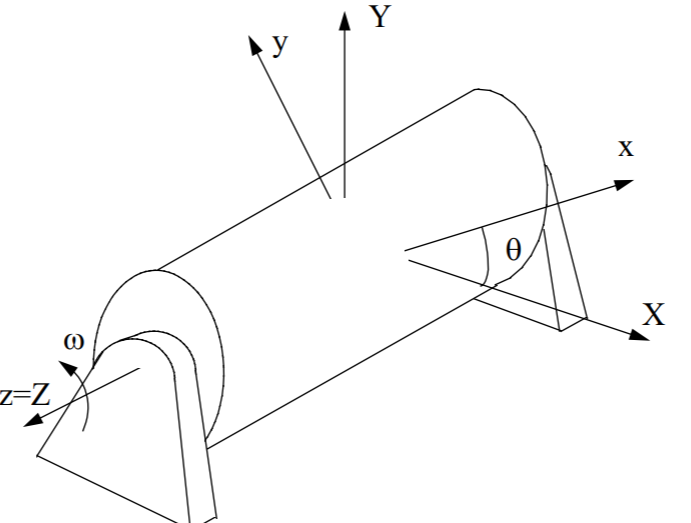
\includegraphics[width=8cm]{C:/Users/patri/Downloads/Poli/lateco/mecanica/figuras/rotor.png}
\end{center}

\subsection{Rotor desbalanceado}

Temos que as equações que configuram o movimento de um rotor desbalanceado são

$$
\begin{cases}

(z_AA_y + z_BB_y) = -(J_{XZ}\ddot{\theta} - J_{YZ}\dot{\theta^2})\\
(z_AA_x + z_BB_x) = -(J_{YZ}\ddot{\theta} - J_{XZ}\dot{\theta^2}) - X_GPsen(\alpha) \\ 
J_Z\ddot{\theta} = H - x_gPcos(\alpha)cos(\theta)

\end{cases}$$

e

$$
\begin{cases}
A_x + B_x = Pcos(\alpha)sen(\theta) - m\dot{\theta}^2x_G \\
A_y + B_y = Pcos(\alpha)cos(\theta) + m\dot{\theta}^2x_g \\
A_z + B_z = Psen(\alpha)

\end{cases}
$$

Onde $\alpha$ é o angulo formado pelo eixo normal ao rotor e a horizontal.
É possível verificar que dados condições de contorno $(\theta, \dot{\theta})$ pode-se integrar as equações acima para encontrar as reações dinâmicas $(A_x, A_y, B_x, B_y)$

\subsection{Rotor balanceado}

\begin{namedtheorem}[Balanceamento Estático]
Centro de massa do sistema deve estar no eixo de rotação do sistema. Com isso, retira-se o momento gerado pelo peso das equações acima.
\end{namedtheorem}

\begin{namedtheorem}[Balanceamento Dinâmico]
Matriz diagonal deve ser nula, portanto deve-se zerar os momentos de inercia, o que irá zerar os termos que multiplicam os momentos de inercia nas equações acima.
\end{namedtheorem}

As equações resultantes são:

$$
\begin{cases}

(z_AA_y + z_BB_y) = 0\\
(z_AA_x + z_BB_x) = 0\\ 
J_Z\ddot{\theta} = H

\end{cases}$$

e

$$
\begin{cases}
A_x + B_x = Pcos(\alpha)sen(\theta)\\
A_y + B_y = Pcos(\alpha)cos(\theta)\\
A_z + B_z = Psen(\alpha)

\end{cases}
$$

\begin{namedtheorem}[Condições de balanceamento]
Portanto as condições de balanceamento são:

\begin{itemize}
	\item $X_g = 0$
	\item $Y_g = 0$
	\item $J_{xz} = 0$
	\item $J_{yz} = 0$
\end{itemize}
\end{namedtheorem}












  \section{Impulso}

As hipóteses assumidas no desenvolvimento da teoria são:

\begin{enumerate}
	\item Enquanto ocorre o \textbf{Impulso} não há variação de posição
	\item Devido o \textbf{Impulso} há variação de velocidade instantânea
	\item Duranto o \textbf{Impulso}, o efeito de outras forças impulsivas são desprezíveis
\end{enumerate}

\begin{namedtheorem}[Definição de Impulso]
$$ \norm{\vec{I}} = \int_{0}^{\delta t} \vec{F}\cdot dt $$
\end{namedtheorem}

\subsection{Teorema da Resultante do Impulso - TRI}

Hipóteses:

\begin{enumerate}
	\item $\vec{r}_i = \vec{r'}_i$
	\item $\vec{\dot{r}}_i \neq \vec{\dot{r'}}_i$
\end{enumerate}

Tem-se que a definição do TRI é:

$$ \boxed{I = m\delta V_g} $$

\subsection{Teorema do Momento de Impulso - TMI}

Definição para partículas

$$\sum_{i=1}^N \vec{r_i}\wedge m_i(\vec{V_{p_i}'} - \vec{V_{p_i}}) = \vec{M_o}$$

Para um corpo rígido

$$m(G-O)\wedge \delta \vec{v_o} + [i,j,k]J_o[\delta \omega] = \vec{M_o}$$

Havendo as classicas simplificações

\begin{enumerate}
	\item $O=G$, quando o polo escolhido for correspondente ao centro de massa
	\item Quando $O$ for um ponto fixo
\end{enumerate}

$$ \boxed{M_o = [i,j,k]J_o\delta\omega_o}  $$

As vezes pode ser interessante na resolução de exercícios considerar o \textit{momento angular} de cada corpo ou considerar o \textit{momento angular total do sistema}. Nesta última opção, o impulso entre corpos é desconsiderado, avalia-se apenas \textit{impulsos externos ao sistema}.

\subsection{Centro de Percussão}

Em algumas situações existem pontos de um corpo em que se forem aplicados \textit{forças impulsivas}, não irá ocorrer uma resposta impulsiva de eventuais articulações deste sistemas. A estes pontos, chamamos de \textbf{Centro de Percussão}. É importante salientar que a \textbf{condição necessária} para que haja um centro de percussão é a de que o corpo esteja rotacionando em relação a um de seus \textbf{eixos principais }, para que os \textbf{produtos de inercia sejam 0}.



  \section{Choque}

\subsection{Hipótese de Newton}

Assumindo a Hipótese de que as superfícies dos corpos nas quais ocorre o choque são lisas, podemos afirmar que apenas a velocidade projetadas na normal de choque sofrerão alteração

\begin{center}
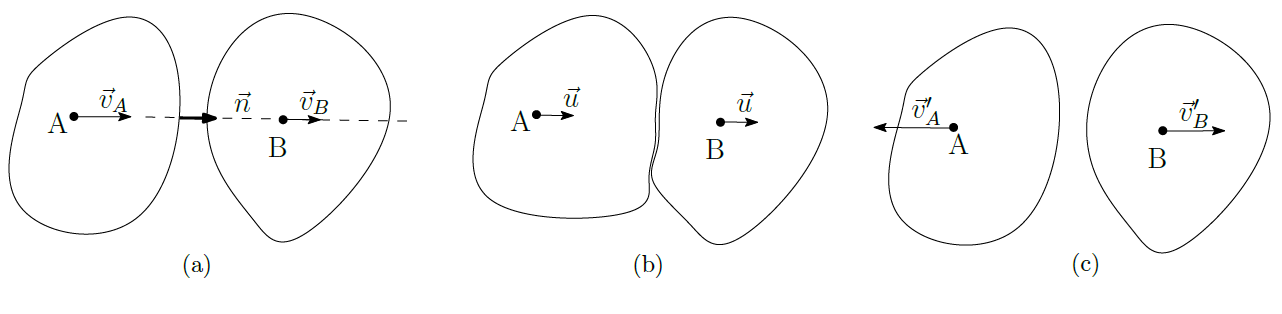
\includegraphics[width=8cm]{C:/Users/patri/Downloads/Poli/lateco/mecanica/figuras/hipotese_choque.png}
\end{center}

Na Hipótese de Newton define-se um \textit{coeficiente de restituição} que é a proporção entre as velocidades do centro de massa dos corpos anteriormente ao choque e posteriormente ao choque

$$ \boxed{V_A' - V_B' = e(V_B - V_A)} $$

O valor deste coeficiente determina o tipo do choque estudado.

\begin{enumerate}
	\item $e = 1$, choque perfeitamente elástico
	\item $0 < e < 1$, choque parcialmente elástico
	\item $e = 0$, choque inelástico
\end{enumerate}

\subsection{Hipótese de Poisson}

A etapa de Poisson divide o choque em duas etapas

\begin{enumerate}
	\item Etapa de Compressão. Haverá compressão das superfície até que as forças Impulsivas igualem as velocidades dos pontos de contato.
	\item Etapa de Restituição. As superfícies se expandem e os corpos se separam.
\end{enumerate}

\begin{center}
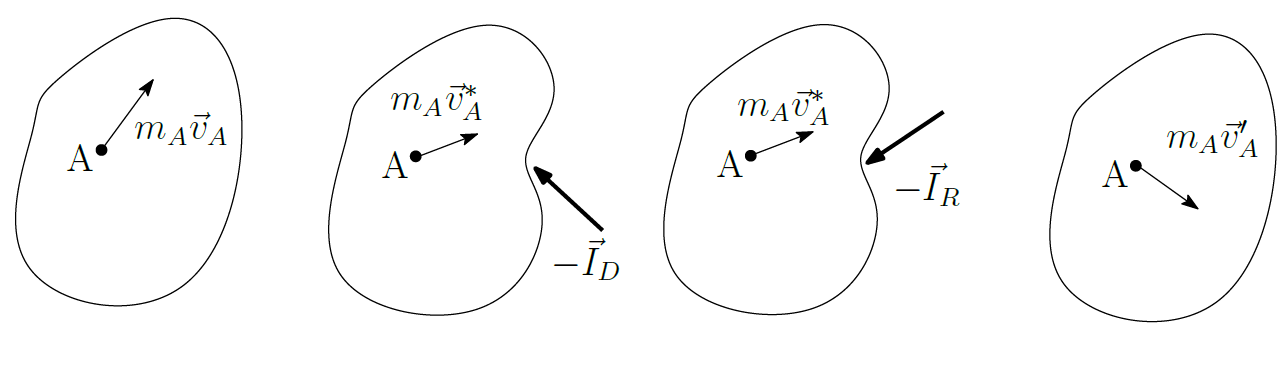
\includegraphics[width=8cm]{C:/Users/patri/Downloads/Poli/lateco/mecanica/figuras/choque_poisson.png}
\end{center}

Onde a direção dos Impulsos sempre será à da normal de choque caso as superfícies sejam adotadas como lisas.

Esta hipótese utiliza do \textit{coeficiente de restituição} para estabelecer a relação entre as velocidades antes do choque e posteriores ao choque.

$$ \boxed{e = \frac{\vec{I_r}\cdot \vec{n}}{\vec{I_D}\cdot \vec{n}} = \frac{V_A' - V_B'}{V_B - V_A}} $$
  \section{Mecanica Analítica introdução}

Definiremos todos os conceitos utilizando o exemplo do pêndulo duplo abaixo.

\subsection{Graus de Liberdade}

Quantidade de coordenadas livres que descrevem o sistema por completo. \\Ou seja no exemplo acima, se sabemos o valor de $\theta_1$ e o valor ed $\theta_2$ sabemos a posição de todos os elementos do pêndulo.

\subsection{Vínculo}

Restrições ao movimento de um corpo.\\
No caso do exemplo, temos dois vínculos, a \textbf{articulação da barra 1} ao teto e a \textbf{articulação da barra 2} que liga ela a barra 1.\\

O vínculos possuem \textbf{equações vínculares}, que são a descrição algébrica da restrição imposta pelo messmo.

No exemplo do pêndulo, caso adotemos as coordenadas do sistema como $(x_1, y_1, x_2, y_2)$, teremos que as equações vinculares seriam:

$\begin{cases} (x_1 - a)^2 + (y_1 - b)^2 = L^2 \\ (x_2 - x_1)^2 + (y_2 - y_1)^2 = L^2 \end{cases}$

No caso teriamos 4 coordenadas, porém 2 equações vinculares, resultando em 2 graus de liberdade.

\begin{namedtheorem}[Vínculo Holônomo Reônomo]
  Vínculos que possuem dependencia do tempo em suas equações.
\end{namedtheorem}

\begin{namedtheorem}[Vínculos Holônomo Esclerônomo]
  Vínculos que não possuem dependência do tempo em suas equações.
\end{namedtheorem}

\begin{namedtheorem}[Vínculos Não Holônomo]
  Vínculos que podem ser expressos apenas em equações diferenciais, cuja integração analítica é impossível.
  Neste tipo de sisema são necessárias mais coordenadas para a descrição da \textit{configuração} do que o número de graus de liberdade, visto que eles não possibilitam eliminar variáveis como equações de \textit{vínculos holônomos}.
\end{namedtheorem}

\subsection{Configuração}

No exemplo acima visualizamos que é possível descrever o mesmo sistema de diversas manerias, poderiamos \\\textbf{(1)} utilizar quatro coordendas $(x_1, y_1, x_2, y_2)$ \\\textbf{(2)} utilizar duas coordenadas $(\theta_1, \theta_2)$

Lançamos mão do conceito de \textit{coordenadas generalizadas}, são as coordenadas independentes do sistema em um determinado sistema, ou seja $(\theta_1, \theta_2)$ seriam coordenadas generalizadas.

E a \textit{configuração} do sistema é equivalente à posição dada pelas \textit{coordenadas generelizadas}, e o conjunto de coordenadas generalizadas define o \textit{espaço da configuração}.

\begin{namedtheorem}[Válidade do espaço de configuração]
Dado uma configuração tal que: \\
$q_1, q_2, \cdots, q_n$ são as coordenadas generalizadas\\
$m$ número de equações vinculares no espaço de coordenadas generalizadas\\
$x_1, x_2, \cdots, x_j$ coordenadas no sistema cartesiano\\
$l$ numero de equações vínculares no sistema cartesiano \\
$f_1, f_2, \cdots, f_j$ funções de transformação de coordenadas generalizadas para o cartesiano\\

Teremos que a configuração é representativa se:

\begin{enumerate}
	\item $GL = n - m = j - l$
	\item $J = |\frac{\partial (f_1, f_2, \cdots, f_j)}{\partial (q_1, q_2, \cdots, q_n)}| \neq 0$
\end{enumerate}

\end{namedtheorem}












  \section{Principio dos trabalhos virtuais}

\begin{center}
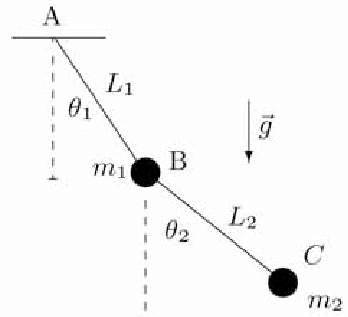
\includegraphics[width=8cm]{C:/Users/patri/Downloads/Poli/lateco/mecanica/figuras/pendulo_duplo.png}
\end{center}

\begin{namedtheorem}[Definição: Trabalho]
O \textbf{trabalho elementar} sobre uma partícula que percorre um caminho é definido como \\
$d\tau = \vec{F}\cdot d\vec{r} = \sum_{i=1}^n \vec{F_i}\cdot d\vec{r_i}$
\end{namedtheorem}

\subsection{Deslocamento Virtual}

É definido como um deslocamento de uma partícula \textit{arbitrariamente pequeno}, em conforme com os vínculos aos quais a partícula estiver sujeita. 

$\delta \vec{x} = \delta x_1 + \delta x_2 + \cdots, + x_N$

Apenas deslocamentos que não desrespeitam as equações dos vínculos são permitidos.


\subsection{Vinculos no deslocamento virtual}

Neste tipo de deslocamento, considera-se que este deslocamento é instantâneo, portanto o tempo é desconsiderado de todas equações, portanto todo vínculos se tornam \textit{esclerônomos}.

$\phi_j(x_1, x_2, \cdots, x_{N}, t) = 0, \textit{  } j =1, \cdots, k$

Diferenciando

$d \phi_j = \sum_{i=1}^{N} \frac{\partial \phi_j}{\partial x_i} + \frac{\partial \phi_j}{\partial t}dt = 0, \textit{  } j=1, \cdots, k$

No deslocamento virtual, tem-se que:

$\partial \phi_j = \sum_{i=1}^{N} \frac{\partial \phi_j}{\partial x_i}, \textit{  } j=1, \cdots, k$

Desta forma, um \textbf{deslocamento virtual}, não necessariamente pode ser convertido para um \textbf{deslocamento virtual}, caso haja algum \textbf{vínculo reônomo}

\subsection{Trabalho Virtual}

A condição \textbf{necessária e suficiente} para um sistema estar em equilibrio é que:

$\delta \tau = \sum_{i=0}^n \vec{F_i}\delta\vec{r_i} = 0 $

Tal fato é especialmente vantajoso para sistemas que há muitos agentes, dispensando o calculo de forças internas para impor condições de equilibrio.
























  \section{Dinâmica}

Conforme visto na seção passada, é possível utilizar os conceitos de \textit{Mecânica Analítica} para resolver problemas de \textbf{estática}, porém agora iremos introduzir o \textit{Princípio de D'Alembert} que permite a resolução de problemas de dinâmica com o mesmo ferramental.

\subsection{Princípio de D'Alambert}

Simplesmente definido como:\\

Das Leis de newton temos que:
$$ \vec{F} = m\vec{a}$$
$$ \vec{F} - m\vec{a} = 0$$

Define-se \textit{Força de Inércia} como $F_I = -m\vec{a}$ \\
$$m\vec{a} = \vec{F_I}$$

\textbf{Principio de D'Alambert}:

\begin{equation}
	\boxed{\vec{F} - F_I = 0}
\end{equation}

A \textit{Força de Inércia} não contribui no movimento da partícula, é chamada de uma força fictícia.

\subsection{Princípio de D'Alambert em um sistema de pontos}

Haverão três forças em jogo:

\begin{enumerate}
	\item Forças externas ao sistema, $\vec{F_{i}}$
	\item Forças de interação entre as partículas, $\vec{f_{ij}}$
	\item Forças de inércia de cada partícula, $F_{I_i}$
\end{enumerate}

Para uma partícula $i$ temos que:

$$ \vec{F_i} + \vec{f_{ij}} + \vec{F_{I_i}} = \vec{0} $$

Para um sistema de particular:

$$ \sum_{i=0}^N\sum_{j=0}^N f_{ij} = 0$$

E da definição do \textit{Princípio de D'Alambert}

\begin{equation}
\sum_{i=0}^N \vec{F_{i}} + \vec{f_{ij}} = 0
\label{principio_d_alambert}
\end{equation}


Portanto enuncia-se o teorema como:\\
\textit{Um sistema de partículas sempre possuirá equilibrio entre suas forças de inercia e as forças externas atuantes neste sistema.}

\subsection{Principio de D'Alambert e o PTV}

As forças externas serão divididas em $\vec{F_i}^a$ que são \textit{forças externas ativas} e $\vec{F_i}^v$ que são \textit{forças externas vinculares}.

Teremos que na situação elucidade na equação \ref{principio_d_alambert}, podemos estabelecer uma situação de "Equilibrio" quando a somatória das forças reais e ficticias são 0, logo podemos utilizar o PTV, com a ideia do trabalho virtual.

\begin{equation}
		\delta \tau = \sum_{i=0}^N (\vec{F_i}^a + \vec{F_i}^v - m_1\ddot{\vec{r_i}})\delta \vec{r_i} = 0
\end{equation}

Por fim teremos que pelo fato do movimento respeitar as equações vinculares:

\begin{equation}
	\sum_{i=0}^N (\vec{F_i}^v = 0
\end{equation}

Logo a forma \textit{lagrangeana} para o \textit{princípio de D'Alambert} é:

\begin{equation}
		\delta \tau = \sum_{i=0}^N (\vec{F_i}^a - m_1\ddot{\vec{r_i}})\delta \vec{r_i} = 0
\end{equation}


  \section{Equações Lagrange}

Considerando deslocamentos compátiveis com os vínculos em um corpo rígido

\subsection{Forças Generalizadas}

O trabalho virtual sendo definido por:

$\delta \tau = (F_1\frac{\partial x_1}{\partial q_1} + F_1\frac{\partial x_2}{\partial q_1} + F_3\frac{\partial x_3}{\partial q_1})\delta q_1 + (F_1\frac{\partial x_1}{\partial q_2} + F_1\frac{\partial x_2}{\partial q_2} + F_3\frac{\partial x_3}{\partial q_2})\delta q_2$

Teremos as \textit{forças generalizadas} são definidas como:

$$Q_1 \coloneqq (F_1\frac{\partial x_1}{\partial q_1} + F_1\frac{\partial x_2}{\partial q_1} + F_3\frac{\partial x_3}{\partial q_1})$$
$$Q_2 \coloneqq (F_1\frac{\partial x_1}{\partial q_2} + F_1\frac{\partial x_2}{\partial q_2} + F_3\frac{\partial x_3}{\partial q_2})$$

Conceitualmente, a força generaliza \textbf{não é uma força}, mas sim uma quantidade que multiplicada por um deslocamento em uma coordenada generalizada fornece o valor do trabalho que uma força ativa produziria naquela coordenada. Apesar de não serem uma força, possuem unidade de força para que multiplicada por um deslocamento forneça unidade de energia.

\subsection{Equações de Lagrange}

$$ \boxed{\frac{d}{dt}(\frac{\partial T}{\partial \dot{q_1}}) - \frac{\partial T}{\partial q_1} = Q_1}$$
$$ \boxed{\frac{d}{dt}(\frac{\partial T}{\partial \dot{q_2}}) - \frac{\partial T}{\partial q_2} = Q_2}$$

\subsection{Trabalho de Potencial conservativo}

O trabalho realizado por uma força conservativa de uma configuração do sistema $P$ até à referência do sistema $P_0$ é definido como a energia potêncial.

$$ V = \int_{P}^{P_0} \sum_{P}^{P_0} $$

$$ V = - \int_{P_0}^{P} \sum_{P}^{P_0} $$

$$ \boxed{\delta \tau = (-\frac{\partial V_1}{\partial x_1})\delta x_1 + (-\frac{\partial V_2}{\partial x_2})\delta x_2 + (-\frac{\partial V_3}{\partial x_3})\delta x_3}$$

\subsection{Equações de Lagrange com função potencial}

$$Q_j = \sum_{i=1}^{3N} (-\frac{\partial V}{\partial x_i}\frac{\partial x_i}{\partial q_j}) = -\frac{\partial V}{\partial q_j} $$

$$ \frac{d}{dt}(\frac{\partial T}{\partial \dot{q_j}}) - \frac{\partial T}{\partial q_j} = Q_j $$

$$ \frac{d}{dt}(\frac{\partial T}{\partial \dot{q_j}}) - \frac{\partial T}{\partial q_j} + \frac{\partial V}{\partial q_j} = 0 $$

$$ \boxed{\frac{d}{dt}(\frac{\partial T}{\partial \dot{q_j}}) - \frac{\partial T - \partial V}{\partial q_j} = 0} $$

\subsection{Força dissipativa}

$$ R = \frac{1}{2} \sum_{i=1}^{3N} c_k\dot{x_i}^2, k=1, \dots N $$

\subsection{Langrange mais geral}

$$ \boxed{\frac{d}{dt}(\frac{\partial T}{\partial \dot{q_j}}) - \frac{\partial T - \partial V}{\partial q_j} + \frac{\partial R}{\partial \dot{q_j}} = Q_{NC}} $$







  \section{Linearização}

As simplificações mais usuais ocorrem nos sistemas que são dos seguintes tipos

\begin{enumerate}
	\item Energia Cinética é dada apenas pelo termo quadrático $T_2$, independe explicitamente do tempo
	\item Sitema Conservativo, foras generalizadas são decorrentes de um potêncial
	\item Vínculos são todos holônomos, portanto a config é dada pelas n coordenadas generalizadas
\end{enumerate}

A energia cinética de um sistema pode ser dividida em três termos

$$ T(q, \dot{q}, t) = T_2 + T_1 + T_0 $$

\begin{namedtheorem}[T_2]

$$ T_2 = \frac{1}{2}\sum_{j=1}^n \sum_{r=1}^n [\sum_{i=1}^{3n} m_k(\frac{\partial x_i}{\partial q_j} \frac{\partial x_i}{\partial q_r})] \dot{q_j} \dot{q_r} $$

Onde define-se

$$ a_{jr} = \sum_{i=1}^{3N} m_k(\frac{\partial x_i}{\partial q_j} \frac{\partial x_i}{\partial q_r}) $$

$$T_2 = \frac{1}{2}\sum_{j=1}^n \sum_{r=1}^n a_{jr}  $$

\end{namedtheorem}

\begin{namedtheorem}[T_1 Centrífugo]
$$ T_1 = \sum_{j=1}^n a_j\dot{q_j} $$

Onde

$$ a_j = \sum_{i=1}^{3N} m_k (\frac{\partial x_i}{\partial q_j} \frac{\partial x_i}{\partial t}) $$

\end{namedtheorem}

\begin{namedtheorem}[T_0 Giroscópico]

$$ T_0 = \frac{1}{2} \sum_{i=1}^{3N} m_k (\frac{\partial x_i}{\partial t})^2 $$

\end{namedtheorem}

A linearização é a aproximação por taylor dos termos em torno de um ponto de equilibrio. Através disto é possível obter equações lineares que vão aproximar o comportamento do sistema em deslocamentos pequenos em relação à este ponto.

$$ \boxed{M_q \ddot{q} + D\dot{u} + K u \approx 0} $$

\begin{namedtheorem}[Matriz da energia cinética]

$$ \boxed{M(q) = [\frac{\partial^2 T}{\partial \dot{q}^2}] = [\frac{\partial^2 T}{\partial \dot{q_i} \partial \dot{q_j}}]} $$

Propriedades:

\begin{itemize}
	\item Matriz simétrica por construção
	\item Matriz de massa
	\item Deve obdecer critérios de ponto de mínimo de uma matriz de derivadas parciais(Matriz hessiana)
	$$ det K > 0 $$
	\item Existem casos em que esta matriz pode ser positiva semi-definida, exigindo tratamento especial
\end{itemize}

\end{namedtheorem}

\begin{namedtheorem}[Matriz da energia potencial]

$$ \boxed{K = [\frac{\partial^2 V}{\partial q^2}] = [\frac{\partial^2 V}{\partial q_i \partial q_j}]} $$

Propriedades:

\begin{itemize}
	\item Matriz simétrica por construção
	\item Matriz de rigidez
	\item Deve obdecer critérios de ponto de mínimo de uma matriz de derivadas parciais(Matriz hessiana)
	$$ det K > 0 $$
\end{itemize}

\end{namedtheorem}

\begin{namedtheorem}[Matriz de amortecimento]

$$ \boxed{D = [\frac{\partial^2 R}{\partial q^2}] = [\frac{\partial^2 R}{\partial q_i \partial q_j}]} $$

Propriedades:

\begin{itemize}
	\item Matriz simétrica por construção
	\item Matriz de Amortecimento
	\item Deve obdecer critérios de ponto de mínimo de uma matriz de derivadas parciais(Matriz hessiana)
	$$ det K > 0 $$
\end{itemize}

\end{namedtheorem}

\begin{namedtheorem}[Condições de Equilibrio]

$$ \boxed{\frac{\partial V}{\partial q_i} = 0} $$

\begin{enumerate}
	\item Se a matriz hessiana da energia potencial for positiva definida, o ponto será de equilibrio estável
	\item Se a matriz hessiana for positiva semi-definida, o ponto será de cela
	\item Se a matriz hessiana for negativa, o equilibrio será instavel no ponto de estudo
\end{enumerate}

\end{namedtheorem}
  
\end{document}